% Provenance (never printed): see sources/outline_sources.md (Year 1:
% geological cross-sections, apparent dip, thickness, boreholes). Every
% Varden Hills number comes from figdata/bachelor-1/varden_sections.py, which
% imports the shared model figdata/shared/region.py; numbers of the exercises
% and problem in the Book 3 scratch calculator and in that script's values.
\chapter{地质剖面图}\label{ch:b1:cross-sections}

一家工程公司计划在瓦尔登丘陵之下修建一条隧道，
自西向东笔直穿过，\omterm{def:b1:spherical-astronomy:horizontal}{海拔}恒定为 \qty{200}{m}。在掘进任何一米之前，
地质学家必须说明掘进机将切过哪些岩层、在何处
穿越断层，以及将在石灰岩中耗费多长时间。石灰岩是一种
可能含有空洞与地下水的岩石。丘陵内部无法直接看到；但
\cref{ch:b1:geological-maps}中的\omterm{def:b1:geological-maps:geological-map}{地质图}、少量钻孔以及
平面的几何关系，便足以在地下画出竖直切面——
即\omterm{def:b1:cross-sections:section}{地质剖面图}——并由此读出答案。本章讲授如何由地图
绘制剖面，切面斜交时\omterm{def:b1:geological-maps:attitude}{倾角}与厚度如何变化，
钻孔如何对比，以及剖面如何讲述
所切岩层的历史。最后回到隧道。

\begin{recall}
平面的\omterm{def:b1:geological-maps:attitude}{产状}由其\omterm{def:b1:geological-maps:attitude}{倾向} $\alpha$ 与\omterm{def:b1:geological-maps:attitude}{倾角}
$\delta$ 给出；过原点处高程为 $z_0$ 的点的平面为
$z = z_0 - \tan\delta\,(x\sin\alpha + y\cos\alpha)$；由接触线上的三点
可确定其\omterm{def:b1:geological-maps:attitude}{产状}；V 形法则根据河谷中的\omterm{def:b1:geological-maps:geological-map}{露头}图样读取\omterm{def:b1:geological-maps:attitude}{倾角}
（见\cref{ch:b1:geological-maps}）。等高线连接地形图上
高程相同的点（第 1 册，九年级）。较新的岩层位于
较老的岩层之上，任何切穿某岩层的构造都比该岩层年轻（第 1 册，七年级）。
\end{recall}

\section{从地图到剖面}

\begin{definition}[地质剖面图、地形剖面、垂直放大]\label{def:b1:cross-sections:section}
称\emph{地质剖面图}\index{地质剖面图}为
沿地图上所画直线、穿过地面的竖直平面内，岩石单元与
构造的图件。其上边缘为
\emph{地形剖面}\index{地形剖面}，即沿该线的地面高程曲线。
其\emph{垂直
放大}\index{垂直放大} $e$ 为剖面的
垂直比例尺与水平比例尺之比；剖面称为\emph{按真实
比例}，即 $e = 1$ 时。
\end{definition}

\begin{method}[由地图绘制地质剖面]\label{met:b1:cross-sections:construct}
\begin{enumerate}
  \item 在地图上画出剖面线，并将一条纸条的边缘沿其放置；
        沿纸条标出各等高线与剖面线的交点，并注明其高程，
        同时标出各接触线与断层的交点。
  \item 画一条与剖面线等长的水平基线，并画出
        高程的竖直比例尺（选定 $e$，并将其写在剖面上）。
  \item 将各等高线的标记转移到相应高程处，并将各点
        光滑连接，即得\omterm{def:b1:cross-sections:section}{地形剖面}。
  \item 将各接触线与断层转移到\omterm{def:b1:cross-sections:section}{地形剖面}上，位置取其与
        剖面线的交点处。
  \item 自每个此类点出发，将接触线按其
        在\emph{剖面平面内}的\omterm{def:b1:geological-maps:attitude}{倾角}——即其\omterm{def:b1:cross-sections:apparent-dip}{视倾角}
        （见\cref{sec:b1:cross-sections:apparent}）——画入地下，按 $e$ 放大，
        若 $e \ne 1$ 时；有钻孔与\omterm{def:b1:cross-sections:structure-contour}{构造等高线}处，应加以利用。
  \item 依据叠置顺序与切割关系，补全各接触线之间的
        岩层单元，并补充图例、比例尺、
        剖面线方向及 $e$。
\end{enumerate}
\end{method}

\begin{omfigure}
\begin{tikzpicture}[font=\scriptsize, x=1cm, y=1cm]
% map strip with contours crossing the section line
\draw[black!50] (0,2.7) rectangle (9,4.5);
\foreach \x/\h in {0.7/300, 1.6/350, 2.6/400, 4.1/400, 5.0/350, 5.8/300, 7.2/300, 8.2/350} {
  \draw[contour, brown!70!black] (\x-0.25,2.7) .. controls (\x+0.1,3.4) and (\x-0.1,3.8) .. (\x+0.2,4.5);
  \node[brown!60!black, above] at (\x+0.2,4.5) {\h};
}
\draw[omThm, thick] (0,3.6) node[left] {X} -- (9,3.6) node[right] {Y};
\fill[omDef] (3.4,3.6) circle (1.5pt);
\node[omDef, fill=white, inner sep=1pt, above right] at (3.4,3.62) {地质界线};
% profile
\draw[->] (0,-0.1) -- (0,1.95) node[above] {高程 (m)};
\draw (0,0) -- (9,0);
\foreach \y/\l in {0/250, 0.5/300, 1.0/350, 1.5/400} { \draw (-0.08,\y) -- (0,\y); \node[left] at (-0.08,\y) {\l}; }
\coordinate (p1) at (0.85,0.5); \coordinate (p2) at (1.75,1.0); \coordinate (p3) at (2.75,1.5);
\coordinate (p4) at (4.25,1.5); \coordinate (p5) at (5.15,1.0); \coordinate (p6) at (5.95,0.5);
\coordinate (p7) at (7.35,0.5); \coordinate (p8) at (8.35,1.0);
\foreach \i/\x in {1/0.85,2/1.75,3/2.75,4/4.25,5/5.15,6/5.95,7/7.35,8/8.35} {
  \draw[black!35, densely dotted] (\x,3.6) -- (p\i);
  \fill (p\i) circle (1.2pt);
}
\draw[thick] (0,0.2) .. controls (0.5,0.3) .. (p1) .. controls (1.3,0.8) .. (p2) .. controls (2.3,1.35) .. (p3)
  .. controls (3.5,1.85) .. (p4) .. controls (4.7,1.25) .. (p5) .. controls (5.5,0.7) .. (p6)
  .. controls (6.6,0.25) .. (p7) .. controls (7.9,0.75) .. (p8) .. controls (8.7,1.15) .. (9,1.2);
\draw[omDef, densely dotted] (3.4,3.6) -- (3.4,1.72);
\draw[omDef, thick] (3.4,1.72) -- (4.45,0.05);
\node[omDef, below right] at (4.3,-0.02) {地质界线，按其视倾角绘出};
\end{tikzpicture}

{\small 剖面的构建（示意）：各等高线
与线 X--Y 的交点投影至相应高程，以得到
\omterm{def:b1:cross-sections:section}{地形剖面}；穿过该线的接触线投影至
剖面上，按其\omterm{def:b1:cross-sections:apparent-dip}{视倾角}画入地下。}
\end{omfigure}

下图由计算机依据瓦尔登丘陵的模型绘制，
沿剖面线 C--D 绘出，该线正东向横穿地图，位于 $y = \qty{6}{km}$ 处。
图中可见一\omterm{def:b1:geological-maps:fold}{背斜}，其核部的砂岩与基底出露于
$x \approx \qty{3.5}{km}$ 处，\omterm{def:b1:geological-maps:fold}{背斜}两翼为石灰岩与页岩，东侧
\omterm{def:b1:geological-maps:fold}{向斜}中为白垩，并有一条正断层。隧道线位于
\qty{200}{m}，图中还标出了钻孔 B1、B2、B3
（见\cref{sec:b1:cross-sections:boreholes}），均已绘出。

\begin{omfigure}
\begin{tikzpicture}
\begin{axis}[x=1.4cm, y=0.0042cm, xmin=0, xmax=10, ymin=-500, ymax=650,
  axis on top, tick label style={font=\scriptsize}, label style={font=\small},
  xlabel={距 C 点向东的距离 (km)}, ylabel={高程 (m)},
  ytick={-400,-200,0,200,400,600}, clip=true]
\addplot[lith schist, draw=black, line width=0.3pt, even odd rule] table {figdata/out/bachelor-1-varden_sections-cd-unit-schist.dat};
\addplot[lith granite, draw=black, line width=0.3pt, even odd rule] table {figdata/out/bachelor-1-varden_sections-cd-unit-granite.dat};
\addplot[om lith={icsTriassic!35}{om sand}, draw=black, line width=0.3pt, even odd rule] table {figdata/out/bachelor-1-varden_sections-cd-unit-sandstone.dat};
\addplot[om lith={icsJurassic!40}{om limestone}, draw=black, line width=0.3pt, even odd rule] table {figdata/out/bachelor-1-varden_sections-cd-unit-limestone.dat};
\addplot[om lith={icsJurassic!15}{om shale}, draw=black, line width=0.3pt, even odd rule] table {figdata/out/bachelor-1-varden_sections-cd-unit-shale.dat};
\addplot[om lith={icsCretaceous!35}{om limestone}, draw=black, line width=0.3pt, even odd rule] table {figdata/out/bachelor-1-varden_sections-cd-unit-chalk.dat};
\addplot[lith alluvium, draw=black, line width=0.3pt, even odd rule] table {figdata/out/bachelor-1-varden_sections-cd-unit-alluvium.dat};
\addplot[black, line width=0.8pt] table {figdata/out/bachelor-1-varden_sections-cd-ground.dat};
\addplot[fault, line width=1.1pt] table {figdata/out/bachelor-1-varden_sections-cd-fault.dat};
\addplot[omThm, line width=1.4pt] coordinates {(1,200) (9,200)};
\node[omThm, font=\scriptsize, fill=white, inner sep=1pt, below] at (axis cs:8.3,190) {隧道，\qty{200}{m}};
\draw[blue!60!black, line width=0.9pt] (axis cs:1.5,-480) -- (axis cs:1.5,524);
\draw[blue!60!black, line width=0.9pt] (axis cs:3.5,-480) -- (axis cs:3.5,381);
\draw[blue!60!black, line width=0.9pt] (axis cs:5.5,-480) -- (axis cs:5.5,530);
\node[font=\scriptsize, blue!60!black, fill=white, inner sep=1pt] at (axis cs:1.5,-440) {B1};
\node[font=\scriptsize, blue!60!black, fill=white, inner sep=1pt] at (axis cs:3.5,-440) {B2};
\node[font=\scriptsize, blue!60!black, fill=white, inner sep=1pt] at (axis cs:5.5,-440) {B3};
\node[font=\small, above right] at (axis cs:0,650) {C（西）};
\node[font=\small, above left] at (axis cs:10,650) {D（东）};
\end{axis}
\end{tikzpicture}

\smallskip
\begin{tikzpicture}
\begin{axis}[x=1.4cm, y=0.0014cm, xmin=0, xmax=10, ymin=-500, ymax=650,
  axis on top, tick label style={font=\scriptsize}, ytick={-500,0,500},
  xticklabels={}, clip=true]
\addplot[lith schist, draw=black, line width=0.2pt, even odd rule] table {figdata/out/bachelor-1-varden_sections-cd-unit-schist.dat};
\addplot[lith granite, draw=black, line width=0.2pt, even odd rule] table {figdata/out/bachelor-1-varden_sections-cd-unit-granite.dat};
\addplot[om lith={icsTriassic!35}{om sand}, draw=black, line width=0.2pt, even odd rule] table {figdata/out/bachelor-1-varden_sections-cd-unit-sandstone.dat};
\addplot[om lith={icsJurassic!40}{om limestone}, draw=black, line width=0.2pt, even odd rule] table {figdata/out/bachelor-1-varden_sections-cd-unit-limestone.dat};
\addplot[om lith={icsJurassic!15}{om shale}, draw=black, line width=0.2pt, even odd rule] table {figdata/out/bachelor-1-varden_sections-cd-unit-shale.dat};
\addplot[om lith={icsCretaceous!35}{om limestone}, draw=black, line width=0.2pt, even odd rule] table {figdata/out/bachelor-1-varden_sections-cd-unit-chalk.dat};
\addplot[lith alluvium, draw=black, line width=0.2pt, even odd rule] table {figdata/out/bachelor-1-varden_sections-cd-unit-alluvium.dat};
\addplot[black, line width=0.6pt] table {figdata/out/bachelor-1-varden_sections-cd-ground.dat};
\addplot[fault, line width=0.8pt] table {figdata/out/bachelor-1-varden_sections-cd-fault.dat};
\end{axis}
\end{tikzpicture}

{\small 沿瓦尔登丘陵的 C--D 剖面，取自该地区的模型。
上：\omterm{def:b1:cross-sections:section}{垂直放大} $e = 3$；下：同一剖面按真实比例
（$e = 1$），此时 \ang{12} 的翼看起来与实际一样平缓。颜色与
\cref{ch:b1:geological-maps}中的\omterm{def:b1:geological-maps:geological-map}{地质图}一致；断层（粗线）
为正断层，其东侧断块为下降盘。红线为
习题中的隧道；B1--B3 为钻孔。}
\end{omfigure}

\omterm{def:b1:cross-sections:section}{垂直放大}使薄层与平缓的地形起伏清晰可辨，但它
歪曲了每个角度：\omterm{def:b1:geological-maps:fold}{褶皱}的 \ang{12} 翼在上方剖面中
约显示为 \ang{32}。下一节将精确说明其规律。

\section{视倾角}\label{sec:b1:cross-sections:apparent}

\begin{definition}[视倾角]\label{def:b1:cross-sections:apparent-dip}
平面在给定竖直剖面中的\emph{视倾角}\index{视倾角} $\beta$ 是
水平面与该平面在该剖面中的迹线之间的夹角。
当剖面沿\omterm{def:b1:geological-maps:attitude}{倾向}方向时，它等于真\omterm{def:b1:geological-maps:attitude}{倾角} $\delta$，
沿\omterm{def:b1:geological-maps:attitude}{走向}时则为零。
\end{definition}

\begin{theorem}[视倾角]\label{thm:b1:cross-sections:apparent-dip}
设\omterm{def:b1:geological-maps:attitude}{倾角}为 $\delta$、\omterm{def:b1:geological-maps:attitude}{倾向}为 $\alpha$ 的平面，被竖直剖面截切，
剖面\omterm{def:b1:spherical-astronomy:horizontal}{方位角}为 $\theta$，则该剖面中的\omterm{def:b1:cross-sections:apparent-dip}{视倾角} $\beta$ 满足
\[
  \tan\beta = \tan\delta\,\cos\gamma, \qquad \gamma = \alpha - \theta ,
\]
平面沿方向 $\theta$ 下降，当 $\cos\gamma > 0$ 时。
特别地，$|\beta| \le \delta$，等号仅在
沿\omterm{def:b1:geological-maps:attitude}{倾向}方向时成立。
\end{theorem}

\begin{proof}
取平面 $z = z_0 - \tan\delta\,(x\sin\alpha + y\cos\alpha)$，
即\cref{ch:b1:geological-maps}中的平面。沿剖面，长为
$s$、沿方向 $\theta$ 的水平步长对应 $(x, y) = s(\sin\theta, \cos\theta)$，于是
$z = z_0 - s\tan\delta\,(\sin\theta\sin\alpha + \cos\theta\cos\alpha) =
z_0 - s\tan\delta\cos(\alpha - \theta)$。迹线为直线，
沿水平方向每单位距离下降 $\tan\delta\cos\gamma$，即
$\tan\beta$。由于 $|\cos\gamma| \le 1$，故 $|\tan\beta| \le \tan\delta$。
\end{proof}

\begin{omfigure}
\begin{tikzpicture}[font=\scriptsize, x={(1cm,0cm)}, y={(0.6cm,0.45cm)}, z={(0cm,1cm)}]
% hidden edges of the block
\draw[black!30, densely dashed] (0,0,0) -- (0,3,0) -- (4,3,0);
\draw[black!30, densely dashed] (0,3,0) -- (0,3,2);
% the oblique vertical section, from the front-left corner to the back-right one
\fill[black!10, opacity=0.7] (0,0,0) -- (4,3,0) -- (4,3,2) -- (0,0,2) -- cycle;
\draw[black!45] (0,0,0) -- (4,3,0) -- (4,3,2);
% the dipping plane, from the top-west edge down to the base
\fill[omDef!25, opacity=0.75] (0,0,2) -- (2.6,0,0) -- (2.6,3,0) -- (0,3,2) -- cycle;
\draw[omDef] (2.6,0,0) -- (2.6,3,0);
\draw[omDef, very thick] (0,0,2) -- (2.6,0,0);
\draw[omThm, very thick] (0,0,2) -- (2.6,1.95,0);
% visible edges of the block
\draw[black!70] (0,0,0) -- (4,0,0) -- (4,0,2) -- (0,0,2) -- cycle;
\draw[black!70] (0,0,2) -- (0,3,2) -- (4,3,2) -- (4,0,2);
\draw[black!70] (4,0,0) -- (4,3,0) -- (4,3,2);
% labels
\draw[omDef] (2.0,0,0) arc[start angle=180, end angle=142.4, radius=0.6cm];
\node[omDef] at (1.7,0,0.2) {$\delta$};
\node[omDef, below, align=center] at (1.3,0,0) {正面，沿倾向方向：\\ 真倾角 $\delta$};
\node[omThm, right, align=left] at (4.45,2.2,0.3) {斜剖面（灰色）：\\ 视倾角 $\beta < \delta$};
\node[above] at (0,1.5,2) {北};
\draw[->] (0.15,1.5,2.05) -- (0.15,2.2,2.05);
\end{tikzpicture}

{\small \omterm{def:b1:cross-sections:apparent-dip}{视倾角}（示意块体）。一个向东倾斜的平面（蓝色）
在正面（沿\omterm{def:b1:geological-maps:attitude}{倾向}截取的竖直面）上显示真\omterm{def:b1:geological-maps:attitude}{倾角} $\delta$；
在斜切的灰色竖直剖面上，其迹线（红色）
较缓，\omterm{def:b1:cross-sections:apparent-dip}{视倾角}为 $\beta$；在沿\omterm{def:b1:geological-maps:attitude}{走向}（南北向）的
剖面上，它将是水平的。}
\end{omfigure}

\begin{proposition}[垂直放大剖面中的角度]\label{prop:b1:cross-sections:exaggeration}
在\omterm{def:b1:cross-sections:section}{垂直放大}倍数为 $e$ 的剖面中，\omterm{def:b1:cross-sections:apparent-dip}{视倾角}为
$\beta$ 的直线以角 $\beta'$ 绘出，满足 $\tan\beta' = e\tan\beta$。
\end{proposition}

\begin{proof}
沿水平距离 $s$，该直线下降 $s\tan\beta$；
按竖直比例尺为水平比例尺的 $e$ 倍绘制时，下降量在图上显示为
$es\tan\beta$，而图上水平长度同为 $s$。
\end{proof}

\begin{example}
瓦尔登\omterm{def:b1:geological-maps:fold}{背斜}东翼的\omterm{def:b1:geological-maps:attitude}{倾角}为 \ang{12.16}，\omterm{def:b1:geological-maps:attitude}{倾向}为 \ang{080.7}
（见\cref{ch:b1:geological-maps}）。在东西向剖面 C--D 中，
$\gamma = \ang{80.7} - \ang{90} = \ang{-9.3}$，且 $\tan\beta =
\tan\ang{12.16}\cos\ang{9.3} = 0.2154\times0.9868 = 0.2126$：$\beta =
\ang{12.0}$。以 $e = 3$ 绘制时，它显示为 $\arctan(3\times0.2126) =
\ang{32.5}$。在\omterm{def:b1:spherical-astronomy:horizontal}{方位角}为 \ang{071.6} 的剖面 A--B 中，$\gamma = \ang{9.1}$
同样 $\beta = \ang{12.0}$：两条剖面都
接近\omterm{def:b1:geological-maps:attitude}{倾向}方向。断层\omterm{def:b1:geological-maps:attitude}{倾角}为 \ang{60}，\omterm{def:b1:geological-maps:attitude}{倾向}为 \ang{120}，在 C--D 中的
\omterm{def:b1:cross-sections:apparent-dip}{视倾角}为 $\arctan(\tan\ang{60}\cos\ang{30}) = \arctan 1.5 = \ang{56.3}$。
\end{example}

\section{厚度}

\begin{definition}[真厚度，铅直厚度]\label{def:b1:cross-sections:thickness}
岩层的\emph{真厚度}\index{真厚度} $t$ 是其底面与顶面之间
沿与层面垂直方向量得的距离。其\emph{铅直厚度}\index{铅直厚度} $h$ 是
沿铅直方向量得的同一距离，
即竖直钻孔穿过该岩层的长度。
\end{definition}

\begin{proposition}[倾斜岩层的厚度]\label{prop:b1:cross-sections:thickness}
对\omterm{def:b1:geological-maps:attitude}{倾角}为 $\delta$ 的岩层：
\begin{enumerate}
  \item $t = h\cos\delta$；
  \item 在水平地面上，若岩层\omterm{def:b1:geological-maps:geological-map}{露头}的宽度为 $w$，
        沿垂直于\omterm{def:b1:geological-maps:attitude}{走向}的方向量取，则 $t = w\sin\delta$；
  \item 当地面以\omterm{def:b1:geological-maps:attitude}{倾角} $\sigma$ 沿垂直于\omterm{def:b1:geological-maps:attitude}{走向}的方向倾斜时，
        且 $w$ 沿地面量取，
        若地面的倾斜方向与\omterm{def:b1:geological-maps:attitude}{倾向}相反，则 $t = w\sin(\delta + \sigma)$；
        若地面与\omterm{def:b1:geological-maps:attitude}{倾向}同向，则 $t = w\sin(\delta - \sigma)$，
        且其坡度小于岩层\omterm{def:b1:geological-maps:attitude}{倾角}。
\end{enumerate}
\end{proposition}

\begin{proof}
在垂直于\omterm{def:b1:geological-maps:attitude}{走向}的铅直面内，岩层的底面与顶面
是两条\omterm{def:b1:geological-maps:attitude}{倾角}为 $\delta$ 的平行线，二者相距 $t$。
(1) 连接二者的铅直线段与它们的公法线成 $\delta$ 角，
故 $t = h\cos\delta$。(2)--(3) 沿地面连接二者、长度为 $w$ 的线段
与层面所成的角，在地面水平时为 $\delta$，
在地面朝\omterm{def:b1:geological-maps:attitude}{倾向}的反方向升高时为 $\delta + \sigma$（两\omterm{def:b1:geological-maps:attitude}{倾角}相加），
而地面同向下降时为 $\delta - \sigma$，
两平行线间的距离等于该线段长度
乘以该角的正弦。
\end{proof}

\begin{omfigure}
\begin{tikzpicture}[font=\scriptsize]
\pgfmathsetmacro{\d}{25}\pgfmathsetmacro{\t}{1.3}
\pgfmathsetmacro{\h}{\t/cos(\d)}\pgfmathsetmacro{\w}{\t/sin(\d)}
\pgfmathsetmacro{\X}{4.0}
\fill[icsJurassic!30] (-\w,0) -- (0,0) -- (\X,{-\X*tan(\d)}) -- (\X,{-\X*tan(\d)-\h}) -- cycle;
\draw[thick] (0,0) -- (\X,{-\X*tan(\d)}) node[right] {岩层顶面};
\draw[thick] (-\w,0) -- (\X,{-\X*tan(\d)-\h}) node[right] {底面};
\draw[black!70] ({-\w-0.8},0) -- (\X+0.6,0) node[right] {水平地面};
% vertical thickness
\draw[omThm, thick, <->] (1.0,{-1.0*tan(\d)}) -- (1.0,{-1.0*tan(\d)-\h});
\node[omThm, right] at (1.0,{-1.0*tan(\d)-0.55*\h}) {$h$};
% true thickness, perpendicular to the bedding
\coordinate (A) at (2.8,{-2.8*tan(\d)});
\draw[omDef, thick, <->] (A) -- ++({-90-\d}:\t);
\node[omDef, right] at ($(A)+({-90-\d}:0.5*\t)$) {$t$};
% outcrop width on flat ground
\draw[black, thick, <->] (-\w,0.2) -- (0,0.2);
\node[above] at ({-0.5*\w},0.2) {$w$};
\draw[omThm] (1.0,0) arc[start angle=0, end angle=-\d, radius=1.0];
\node[omThm] at (1.25,-0.22) {$\delta$};
\end{tikzpicture}

{\small 垂直于\omterm{def:b1:geological-maps:attitude}{走向}的铅直面内倾斜岩层的厚度：
\omterm{def:b1:cross-sections:thickness}{真厚度} $t$，垂直于层面；
\omterm{def:b1:cross-sections:thickness}{铅直厚度} $h = t/\cos\delta$；\omterm{def:b1:geological-maps:geological-map}{露头}宽度 $w = t/\sin\delta$，
位于水平地面上（示意图，取 $\delta = \ang{25}$）。}
\end{omfigure}

在瓦尔登丘陵，一口自上而下钻入石灰岩的钻孔，穿过该层的岩芯长度为
\qty{180}{m}，此即其\omterm{def:b1:cross-sections:thickness}{铅直厚度}。其\omterm{def:b1:cross-sections:thickness}{真厚度}为
$180\cos\ang{12.16} = \qty{176.0}{m}$。薄层与厚层若\omterm{def:b1:geological-maps:attitude}{倾角}不同，可具有相同的\omterm{def:b1:geological-maps:geological-map}{露头}宽度，
陡倾的岩层在与之同向的坡面上可能显示出较宽的\omterm{def:b1:geological-maps:geological-map}{露头}：
厚度绝不能
直接从地图上读出。

\section{钻孔与构造等高线}\label{sec:b1:cross-sections:boreholes}

\begin{definition}[钻孔柱状图，对比]\label{def:b1:cross-sections:log}
一份\emph{钻孔柱状图}\index{钻孔柱状图}是按深度记录的
钻孔所穿遇岩石的记录：包括各岩层单元、其接触面的深度，以及
任何实测属性。\emph{对比}\index{对比（柱状图）}是
在不同柱状图之间，对应相同岩层单元与接触面的匹配。
\end{definition}

沿剖面 C--D 布设的三口钻孔，给出以下各岩层底面
在地面以下的深度（“——”表示该接触面位于地面以上，
已被侵蚀）：
\begin{center}
\small
\begin{tabular}{lcccccc}
\hline
钻孔 & $x$（km） & 地面（m） & 白垩 & 页岩 & 石灰岩 & 砂岩 \\
\hline
B1 & 1.5 & 524.02 & 388.98 & 488.98 & 668.98 & 788.98 \\
B2 & 3.5 & 380.64 & --- & --- & 100.48 & 220.48 \\
B3 & 5.5 & 529.98 & 394.93 & 494.93 & 674.93 & 794.93 \\
\hline
\end{tabular}
\end{center}
B2 始于石灰岩中，位于\omterm{def:b1:geological-maps:fold}{背斜}的顶部；B1 与 B3 始于
白垩中，位于其两翼。由地面高程减去深度，即得
各接触面的高程：石灰岩底面位于
B2 中为 $380.64 - 100.48 = \qty{280.16}{m}$，在 B3 中为 $529.98 - 674.93 =
\qty{-144.95}{m}$，两者相差 \qty{425.11}{m}，水平距离 \qty{2}{km}，坡度为
\num{0.2126}，即上文求得的\omterm{def:b1:cross-sections:apparent-dip}{视倾角} \ang{12.0}。B1 与 B3 给出的
厚度相同：页岩 \qty{100}{m}，石灰岩 \qty{180}{m}，以及
砂岩 \qty{120}{m}：各岩层单元在两翼上的
\omterm{def:b1:cross-sections:thickness}{铅直厚度}相同。

\begin{omfigure}
\begin{tikzpicture}[font=\scriptsize, x=1cm, y=0.0045cm]
\foreach \b/\xx/\g/\c/\s/\l/\sd in {B1/0/524.02/388.98/488.98/668.98/788.98, B3/6/529.98/394.93/494.93/674.93/794.93} {
  \begin{scope}[xshift=\xx cm]
  \fill[icsCretaceous!35] (0,{\g}) rectangle (0.9,{\g-\c});
  \fill[icsJurassic!15] (0,{\g-\c}) rectangle (0.9,{\g-\s});
  \fill[icsJurassic!40] (0,{\g-\s}) rectangle (0.9,{\g-\l});
  \fill[icsTriassic!35] (0,{\g-\l}) rectangle (0.9,{\g-\sd});
  \fill[black!15] (0,{\g-\sd}) rectangle (0.9,{\g-\sd-40});
  \draw (0,{\g}) rectangle (0.9,{\g-\sd-40});
  \node[above] at (0.45,{\g}) {\b};
  \end{scope}
}
\begin{scope}[xshift=3cm]
  \fill[icsJurassic!40] (0,380.64) rectangle (0.9,280.16);
  \fill[icsTriassic!35] (0,280.16) rectangle (0.9,160.16);
  \fill[black!15] (0,160.16) rectangle (0.9,120);
  \draw (0,380.64) rectangle (0.9,120);
  \node[above] at (0.45,380.64) {B2};
\end{scope}
% correlation lines: base of limestone
\draw[omThm, dashed] (0.9,-144.96) -- (3,280.16);
\draw[omThm, dashed] (3.9,280.16) -- (6,-144.95);
\draw[omDef, dashed] (0.9,-264.96) -- (3,160.16);
\draw[omDef, dashed] (3.9,160.16) -- (6,-264.95);
% elevation axis
\draw[->] (-0.6,-320) -- (-0.6,600) node[above] {高程（m）};
\foreach \y in {-200,0,200,400} { \draw (-0.68,\y) -- (-0.6,\y); \node[left] at (-0.68,\y) {\y}; }
\foreach \c/\yy/\n in {icsCretaceous!35/400/白垩, icsJurassic!15/340/页岩, icsJurassic!40/280/石灰岩, icsTriassic!35/220/砂岩, black!15/160/基底} {
  \fill[\c] (7.2,\yy) rectangle (7.45,\yy+36); \draw (7.2,\yy) rectangle (7.45,\yy+36);
  \node[right] at (7.45,\yy+18) {\n};
}
\node[omThm, right] at (0.95,480) {石灰岩底面};
\node[omDef, left] at (4.0,-250) {砂岩底面};
\end{tikzpicture}

{\small 钻孔 B1、B2 和 B3 的\omterm{def:b1:cross-sections:log}{钻孔柱状图}（沿 C--D 线），按真实高程悬挂排列（非水平比例），及其对比：
石灰岩底面（红色）与砂岩底面（蓝色）自两翼
向上升至 B2 处\omterm{def:b1:geological-maps:fold}{背斜}的
顶部。}
\end{omfigure}

钻孔较多时，埋藏接触面的形状以\omterm{def:b1:cross-sections:structure-contour}{构造等高线}
来刻画。

\begin{definition}[构造等高线，构造等高线图]\label{def:b1:cross-sections:structure-contour}
地质面的\emph{构造等高线}\index{构造等高线}是指
该面上高程相同的各点连成的线。
\emph{构造等高线图}\index{构造等高线图}以规则的间距
绘出某一面的构造等高线，该面可位于地下，
也可已被侵蚀殆尽。
\end{definition}

对于平面，\omterm{def:b1:cross-sections:structure-contour}{构造等高线}为直线，与\omterm{def:b1:geological-maps:attitude}{走向}平行，
且等距分布：等高线之间的高差 $\Delta z$ 对应
的水平间距为 $\Delta z/\tan\delta$。若该面发生\omterm{def:b1:geological-maps:fold}{褶皱}，其
等高线随之弯曲；若断层切穿该面，
等高线便在断层处中断，并错开接续，形成缺口或重叠。

\begin{method}[绘制构造等高线图]\label{met:b1:cross-sections:structure-contours}
\begin{enumerate}
  \item 对每个钻孔，以及该面出露的每一点，
        计算该面的高程（地面高程减去深度；
        在\omterm{def:b1:geological-maps:geological-map}{露头}处则为地面高程本身）。
  \item 若该面近似为平面，则取三点，
        用三点法求出其\omterm{def:b1:geological-maps:attitude}{产状}（见
        \cref{ch:b1:geological-maps}）；沿\omterm{def:b1:geological-maps:attitude}{走向}画出等高线，
        相邻等高线的间距为 $\Delta z/\tan\delta$。
  \item 若不近似为平面，则在相邻点之间作线性插值（以点构成的三角形为单元），
        并连接高程相等的点。
  \item 先画出断层，再对每个断块分别绘制等高线。
\end{enumerate}
\end{method}

\begin{omfigure}
\begin{tikzpicture}
\begin{axis}[axis equal image, xmin=0, xmax=10, ymin=0, ymax=8, width=0.8\linewidth, clip=false,
  tick label style={font=\scriptsize}, xlabel={东 (km)}, ylabel={北 (km)},
  label style={font=\small}]
\addplot[contour, black!25, opacity=0.6] table {figdata/out/shared-region-contours.dat};
\addplot[omThm!80!black, line width=0.6pt] table {figdata/out/bachelor-1-varden_sections-sc.dat};
\addplot[normal fault] table {figdata/out/shared-region-fault.dat};
\addplot[black, densely dashed, line width=0.6pt] coordinates {(0,6) (10,6)};
\node[font=\scriptsize, fill=white, inner sep=1pt, below right] at (axis cs:0.05,5.95) {C};
\node[font=\scriptsize, fill=white, inner sep=1pt, below left] at (axis cs:9.95,5.95) {D};
\addplot[only marks, mark=none, point meta=explicit symbolic, nodes near coords,
  nodes near coords style={font=\tiny, omThm!70!black, fill=white, fill opacity=0.8, text opacity=1, inner sep=0.5pt, anchor=center},
  restrict expr to domain={mod(\thisrow{z_m}+400,200)}{0:0}]
  table[x=x_km, y=y_km, meta=z_m] {figdata/out/bachelor-1-varden_sections-sc-labels.dat};
\pic at (axis cs:10.6,0.8) {northarrow};
\end{axis}
\end{tikzpicture}

{\small 瓦尔登丘陵石灰岩底面的\omterm{def:b1:cross-sections:structure-contour}{构造等高线}，每隔 \qty{100}{m} 一条
（红色，每隔 \qty{200}{m} 标注数值），叠加在地形等高线（灰色）之上。
在两翼，等高线大致沿南北向延伸，与\omterm{def:b1:geological-maps:attitude}{走向}平行；
绕倾伏\omterm{def:b1:geological-maps:fold}{褶皱}的转折端，等高线呈 V 形；
在断层处（短刻线位于下降盘一侧），等高线停于地表的两条截止线，
两截止线之间相隔\omterm{def:b1:cross-sections:throw}{水平断距}，并在上盘错开接续。
剖面 C--D 以虚线表示。}
\end{omfigure}

\section{从剖面到历史}

剖面不仅显示岩石位于何处，还显示它们是如何形成于此的。
各单元之间的接触关系记录了连续沉积，或是一段空缺。

\begin{definition}[不整合，角度不整合，平行不整合]\label{def:b1:cross-sections:unconformity}
\emph{不整合}\index{不整合}是一种侵蚀面或未沉积面，它将较新的岩层
与较老的岩层分隔开，因而标志着地层记录中的一段空缺。
在\emph{角度不整合}\index{角度不整合}中，较老的岩层在
较新的岩层覆于其被侵蚀的边缘之前已倾斜或\omterm{def:b1:geological-maps:fold}{褶皱}，
因而两组岩层以一定夹角相交。在
\emph{平行不整合}\index{平行不整合}中，上下岩层相互平行，
空缺仅表现为侵蚀面，
或表现为化石或年代的缺失。
\end{definition}

\begin{definition}[垂直断距，水平断距]\label{def:b1:cross-sections:throw}
断层的\emph{垂直断距}\index{垂直断距（断层）}是指标志面穿过断层时的位移
在竖直方向上的分量；其\emph{水平断距}\index{水平断距（断层）}为
水平分量，沿断层\omterm{def:b1:geological-maps:attitude}{倾向}方向量取。
对于\omterm{def:b1:geological-maps:attitude}{倾角}为 $\varphi$ 的倾滑断层，
$\text{水平断距} = \text{垂直断距}/\tan\varphi$。
\end{definition}

瓦尔登丘陵的正断层\omterm{def:b1:geological-maps:attitude}{倾角}为 \ang{60}，\omterm{def:b1:cross-sections:throw}{垂直断距}为 
\qty{200}{m}，其\omterm{def:b1:cross-sections:throw}{水平断距}为 $200/\tan\ang{60} = \qty{115.5}{m}$。在剖面
C--D 中（与断层\omterm{def:b1:geological-maps:attitude}{倾向}斜交），断层的\omterm{def:b1:cross-sections:apparent-dip}{视倾角}为
\ang{56.3}，同样的 \qty{200}{m} \omterm{def:b1:cross-sections:throw}{垂直断距}使某一接触界线的两条截止线
沿剖面相隔 $200/1.5 = \qty{133.3}{m}$。要
\emph{复原}剖面——即看到断层移动之前岩石的状态——
应将上盘岩块沿断层面向上滑回一个滑距；
若同时将\omterm{def:b1:geological-maps:fold}{褶皱}复原，即将岩层展平，
则可恢复被侵蚀基底之上平卧的盖层。从下往上读剖面，
瓦尔登丘陵的历史依次为：片岩、侵入其中的花岗岩、侵蚀、
\omterm{def:b1:cross-sections:unconformity}{角度不整合}、平卧盖层的沉积、\omterm{def:b1:geological-maps:fold}{褶皱}、断裂，
以及形成今日丘陵的侵蚀作用。

\begin{history}[赫顿在锡卡尔角]
% ledger: iugs:siccar-point
锡卡尔角位于苏格兰东南海岸，近乎直立的
灰色砂岩与泥岩（早志留世）被一个侵蚀面切断，其上
覆盖着平缓倾斜的红色角砾岩、砾岩和砂岩（晚泥盆世）。
詹姆斯·赫顿在其 \emph{Theory of the Earth} 中描述了这一\omterm{def:b1:cross-sections:unconformity}{角度不整合}，
该书于 1788 年宣读于爱丁堡皇家学会，并刊印于 \emph{Transactions}，
随后于 1795 年扩充成书出版；詹姆斯·霍尔爵士所绘的草图
记录了赫顿所见。下层岩层原本
平铺于海底，后被抬起竖立、升高并遭受剥蚀；
此后才有上层岩层沉积其上，整体再次抬升。每一步都需要
远比人们此前所设想的长得多的时间，
赫顿对这一\omterm{def:b1:geological-maps:geological-map}{露头}的解读，
常被视为地质学认识到地球年龄的时刻。
\begin{center}
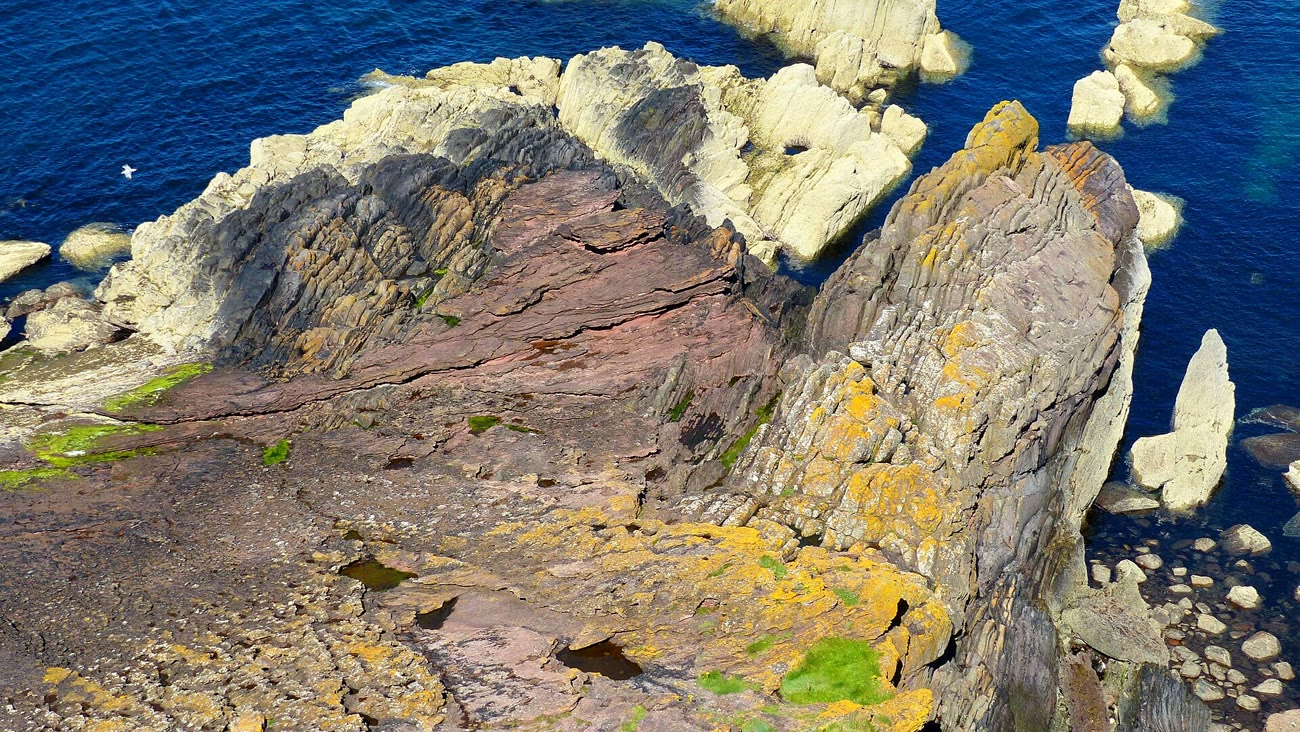
\includegraphics[width=0.7\linewidth]{images/book3/b1-siccar-point.jpg}

{\small 赫顿在锡卡尔角的\omterm{def:b1:cross-sections:unconformity}{不整合}：下方为近乎直立的灰色志留纪岩层，
上方为缓倾的红色泥盆纪岩层。照片：PawełS，
CC BY-SA 4.0（维基共享资源）。}
% ledger: commons:siccar-point
\end{center}
\end{history}

\begin{inthefield}[隧道工程中的地质]
\begin{minipage}[t]{0.6\linewidth}\vspace{0pt}
在隧道设计之前，工程地质学家沿隧道线路
依据\omterm{def:b1:geological-maps:geological-map}{地质图}、沿线按间隔布置的钻孔以及地球物理勘探，
编制地质剖面。他们预测隧道将穿过的每一地层单元，
将跨越的断层，以及水可能涌入的部位。掘进期间，
施工承包方的地质人员在每次推进时记录掌子面出露的岩石，
并与预测相比较，修订剖面；
在掘进机前方钻设的探孔，在掘进机到达之前检测地层，
尤其是在预测断层附近，或在可能含有溶洞的石灰岩中。
断层破碎带是典型的灾害，
尤其当两侧为相同岩性、掌子面上无任何迹象预警时。
\end{minipage}\hfill
\begin{minipage}[t]{0.37\linewidth}\vspace{0pt}
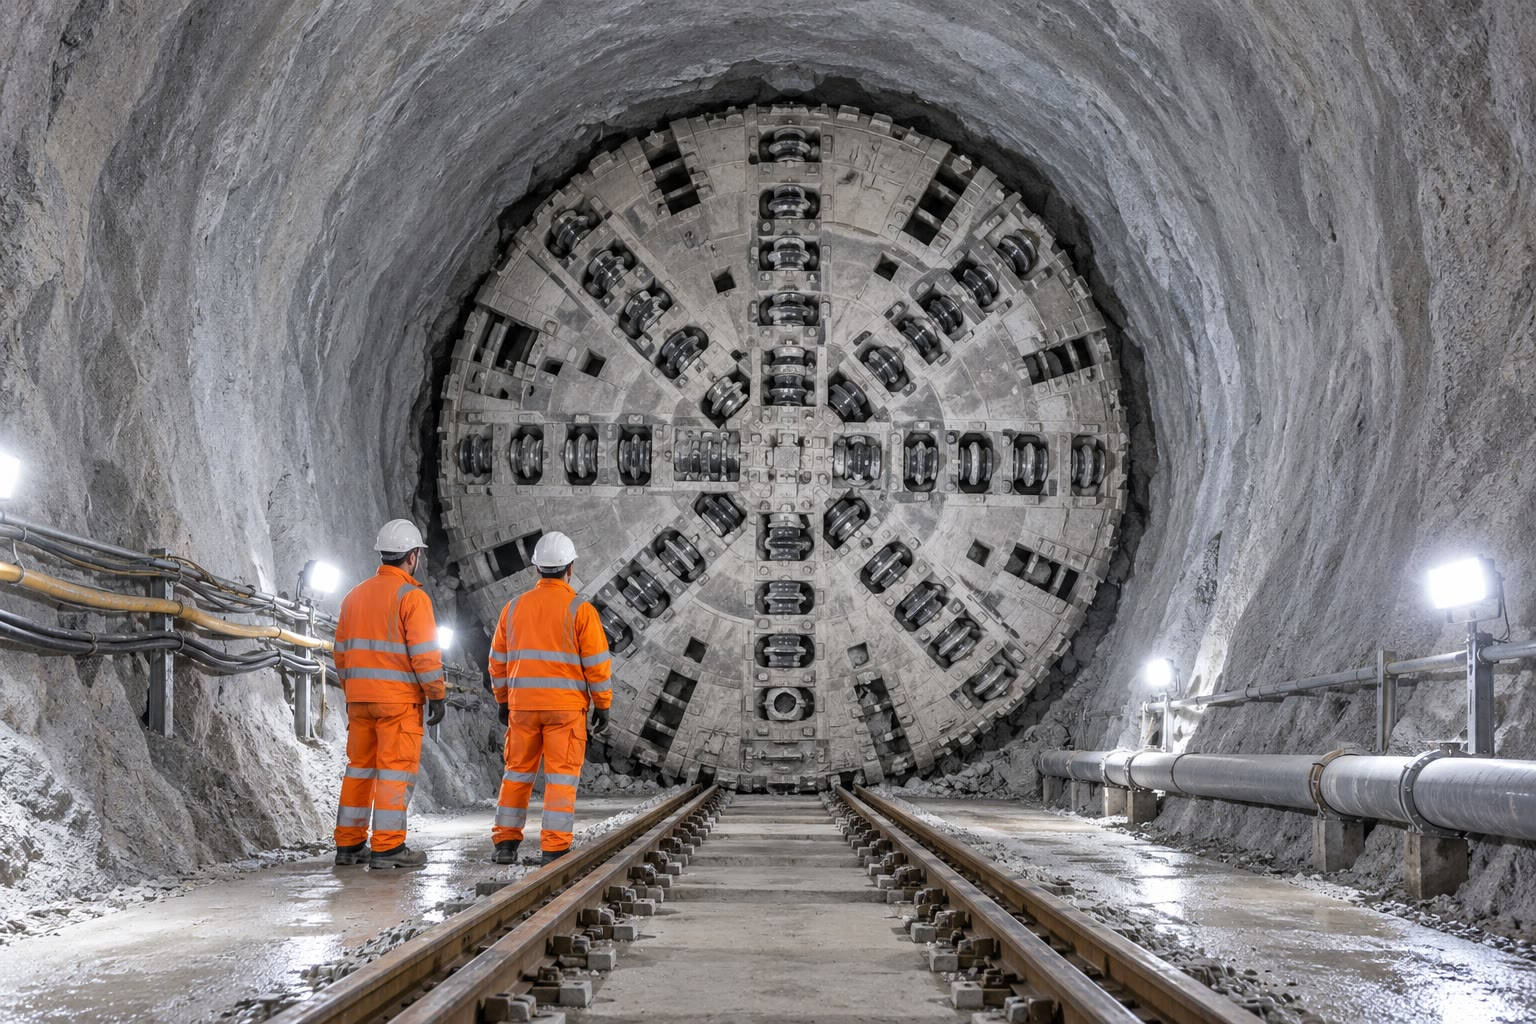
\includegraphics[width=\linewidth]{images/book3/ai/b1-tunnel-boring.jpg}
\end{minipage}
\end{inthefield}

\section{练习}

\begin{exercise}[$\star$]\label{exo:b1:cross-sections:1}
由比例尺为 1:25\,000 的地图绘制一剖面，竖直比例尺为
\qty{1}{cm} 代表 \qty{100}{m}。求其\omterm{def:b1:cross-sections:section}{垂直放大}。
\end{exercise}

\begin{exercise}[$\star$]\label{exo:b1:cross-sections:2}
某岩层\omterm{def:b1:geological-maps:attitude}{倾角}为 \ang{40}，\omterm{def:b1:geological-maps:attitude}{倾向}为 \ang{090}。求其在\omterm{def:b1:spherical-astronomy:horizontal}{方位角}为 \ang{060} 的竖直剖面中的\omterm{def:b1:cross-sections:apparent-dip}{视倾角}，
以及\omterm{def:b1:spherical-astronomy:horizontal}{方位角}为 \ang{000} 的剖面中的\omterm{def:b1:cross-sections:apparent-dip}{视倾角}？
\end{exercise}

\begin{exercise}[$\star$]\label{exo:b1:cross-sections:3}
一竖直钻孔穿过厚 \qty{120}{m} 的砂岩，其岩层\omterm{def:b1:geological-maps:attitude}{倾角}为
\ang{12.16}。求该砂岩的\omterm{def:b1:cross-sections:thickness}{真厚度}。
\end{exercise}

\begin{exercise}[$\star$]\label{exo:b1:cross-sections:4}
某接触面位于剖面平面内，\omterm{def:b1:geological-maps:attitude}{倾角}为 \ang{12}，分别以\omterm{def:b1:cross-sections:section}{垂直放大} 2、3 和 5 绘制，
求其在图中显示的角度分别为多少？
\end{exercise}

\begin{exercise}[$\star\star$]\label{exo:b1:cross-sections:5}
某岩层\omterm{def:b1:geological-maps:attitude}{倾角}为 \ang{25}。其\omterm{def:b1:geological-maps:geological-map}{露头}宽 \qty{300}{m}，
沿垂直于\omterm{def:b1:geological-maps:attitude}{走向}的方向测得。求其\omterm{def:b1:cross-sections:thickness}{真厚度}：(a) 在平坦地面上；
(b) 地面以 \ang{10} 的坡度向与\omterm{def:b1:geological-maps:attitude}{倾向}相反的方向倾斜，宽度
沿地面量取；(c) 地面以 \ang{10} 的坡度倾斜，
倾斜方向与\omterm{def:b1:geological-maps:attitude}{倾向}相同。
\end{exercise}

\begin{exercise}[$\star\star$]\label{exo:b1:cross-sections:6}
某岩层在南北向剖面中的\omterm{def:b1:cross-sections:apparent-dip}{视倾角}为 \ang{20}，指向北，
在东西向剖面中为 \ang{30}，指向东。求其\omterm{def:b1:geological-maps:attitude}{倾向}及
真\omterm{def:b1:geological-maps:attitude}{倾角}。
\end{exercise}

\begin{exercise}[$\star\star$]\label{exo:b1:cross-sections:7}
东翼石灰岩的底面\omterm{def:b1:geological-maps:attitude}{倾角}为 \ang{12.16}。求
\omterm{def:b1:cross-sections:structure-contour}{构造等高线}沿水平方向的间距（每隔 \qty{100}{m} 绘一条）是多少？核对
此值，并在\omterm{def:b1:cross-sections:structure-contour}{构造等高线图}上检验。
\end{exercise}

\begin{exercise}[$\star\star$]\label{exo:b1:cross-sections:8}
根据钻孔表，计算 B1 和 B3 处页岩底面的高程。在 B2 上方，页岩已被剥蚀：
由石灰岩的\omterm{def:b1:cross-sections:thickness}{铅直厚度}，求其底面在该处应有的高程，
以及 B1 与 B2 之间该接触面在 C--D 剖面中的\omterm{def:b1:cross-sections:apparent-dip}{视倾角}。
比较 B1 与 B3 的结果，能说明该\omterm{def:b1:geological-maps:fold}{褶皱}的
什么特征？
\end{exercise}

\begin{exercise}[$\star\star$]\label{exo:b1:cross-sections:9}
一正断层\omterm{def:b1:geological-maps:attitude}{倾角}为 \ang{50}，\omterm{def:b1:geological-maps:attitude}{倾向}为 \ang{180}，其\omterm{def:b1:cross-sections:throw}{垂直断距}为
\qty{150}{m}。求其\omterm{def:b1:cross-sections:throw}{水平断距}。在\omterm{def:b1:spherical-astronomy:horizontal}{方位角}为 \ang{150} 的竖直剖面中，
求该断层的\omterm{def:b1:cross-sections:apparent-dip}{视倾角}，以及沿该剖面一水平岩层两截止线
之间的间距？
\end{exercise}

\begin{exercise}[$\star\star\star$]\label{exo:b1:cross-sections:10}
对于\omterm{def:b1:geological-maps:attitude}{倾角}为 \ang{40} 的岩层，在哪些剖面方向上\omterm{def:b1:cross-sections:apparent-dip}{视倾角}
恰为真\omterm{def:b1:geological-maps:attitude}{倾角}的一半，即 \ang{20}？证明\omterm{def:b1:cross-sections:apparent-dip}{视倾角}在\omterm{def:b1:geological-maps:attitude}{倾向}附近变化
较小，而在\omterm{def:b1:geological-maps:attitude}{走向}附近变化迅速。
\end{exercise}

\begin{exercise}[$\star\star\star$]\label{exo:b1:cross-sections:11}
一钻孔穿过东翼石灰岩（\omterm{def:b1:cross-sections:thickness}{真厚度}
\qty{176.0}{m}，\omterm{def:b1:geological-maps:attitude}{倾角} \ang{12.16}，\omterm{def:b1:geological-maps:attitude}{倾向} \ang{080.7}）。该钻孔取得的岩芯长度为多少
（a）若钻孔竖直；（b）若钻孔与水平面成 \ang{60} 倾斜
并朝 \ang{260.7} 方向向下；（c）若钻孔以 \ang{60} 倾斜并朝 \ang{080.7}？
（提示：长度为 $t/\cos\psi$，其中 $\psi$ 为
钻孔与层面法线的夹角。）
\end{exercise}

\begin{exercise}[$\star\star\star$]\label{exo:b1:cross-sections:12}
在\omterm{def:b1:cross-sections:unconformity}{角度不整合}处，下伏岩层\omterm{def:b1:geological-maps:attitude}{倾角}为 \ang{70}，\omterm{def:b1:geological-maps:attitude}{倾向}为 \ang{090}，
上覆岩层\omterm{def:b1:geological-maps:attitude}{倾角}为 \ang{20}，\omterm{def:b1:geological-maps:attitude}{倾向}为 \ang{270}，二者\omterm{def:b1:geological-maps:attitude}{走向}相同。
绕\omterm{def:b1:geological-maps:attitude}{走向}将整个\omterm{def:b1:geological-maps:geological-map}{露头}旋转，使上覆岩层恢复
水平。问上覆岩层沉积时，
下伏岩层的\omterm{def:b1:geological-maps:attitude}{倾角}为多少？试按顺序写出该\omterm{def:b1:geological-maps:geological-map}{露头}的形成历史。
\end{exercise}

\section{问题：瓦尔登丘陵下的隧道}

\begin{problem}[{周末问题——隧道将穿过哪些岩层，在何处与断层相遇，
以及将掘进多少石灰岩}]
\label{pb:b1:cross-sections:1}
% numbers from figdata/bachelor-1/varden_sections.py (model region.py) and the scratch calculator
隧道沿 C--D 线正东向延伸（$y = \qty{6}{km}$），
高程恒定为 \qty{200}{m}，自 $x = \qty{1}{km}$ 至 $x =
\qty{9}{km}$。沿 C--D 的地面高程自 $x = 0$ 起每隔 \qty{1}{km}
取一值，如下：
\begin{center}
\small
\begin{tabular}{lccccccccccc}
\hline
$x$ (km) & 0 & 1 & 2 & 3 & 4 & 5 & 6 & 7 & 8 & 9 & 10 \\
$z$ (m) & 509 & 556 & 467 & 370 & 435 & 534 & 501 & 455 & 406 & 339 & 405 \\
\hline
\end{tabular}
\end{center}
利用本章的钻孔表、以 $e = 3$ 绘制的 C--D 剖面，
东翼的\omterm{def:b1:geological-maps:attitude}{产状}（\omterm{def:b1:geological-maps:attitude}{倾角} \ang{12.16}，\omterm{def:b1:geological-maps:attitude}{倾向} \ang{080.7}；西翼
为其镜像，\omterm{def:b1:geological-maps:attitude}{倾向} \ang{279.3}），以及正断层，
该断层\omterm{def:b1:geological-maps:attitude}{倾角}为 \ang{60}，\omterm{def:b1:geological-maps:attitude}{倾向}为 \ang{120}，\omterm{def:b1:cross-sections:throw}{垂直断距}为 \qty{200}{m}，并
经过点 $x = \qty{4.30}{km}$，$y = \qty{1.00}{km}$，
$z = \qty{250}{m}$。

\medskip
\noindent\textbf{第一部分——剖面与单位。}
\begin{enumerate}
  \item 在 $x = 1$ 与 $x = 9$ 之间各千米点处，隧道上方岩层的
        最大厚度与最小厚度分别是多少？
  \item 在打印的剖面图上，水平距离 \qty{1}{km} 量得 \qty{1.4}{cm}，
        高程 \qty{1}{km} 量得 \qty{4.2}{cm}。
        验证 $e = 3$。
  \item 由钻孔 B2 求
        \omterm{def:b1:geological-maps:fold}{背斜}顶部砂岩底面的高程。
  \item 隧道在 $x = \qty{3.5}{km}$ 处穿过哪个地层单元？
  \item 计算 B1 和 B3 中石灰岩底面的高程。
  \item 由剖面依次列出隧道从 $x = 1$ 至
        $x = \qty{9}{km}$ 所穿过的地层单元。
\end{enumerate}

\medskip
\noindent\textbf{第二部分——剖面中的\omterm{def:b1:geological-maps:attitude}{倾角}。}
\begin{enumerate}[resume]
  \item 由东翼的\omterm{def:b1:geological-maps:attitude}{产状}，计算 C--D 剖面中东翼的\omterm{def:b1:cross-sections:apparent-dip}{视倾角}。
  \item 由 B2 与 B3 中石灰岩底面的高程，
        验证该结果。
  \item 在 $e = 3$ 的剖面中，东翼是以多大角度画出的？
  \item 计算 C--D 剖面中断层的\omterm{def:b1:cross-sections:apparent-dip}{视倾角}。
  \item 为什么 C--D 剖面中两翼的\omterm{def:b1:cross-sections:apparent-dip}{视倾角}与其真\omterm{def:b1:geological-maps:attitude}{倾角}如此接近，
        而断层的\omterm{def:b1:cross-sections:apparent-dip}{视倾角}与其真\omterm{def:b1:geological-maps:attitude}{倾角}则较为不同？
\end{enumerate}

\medskip
\noindent\textbf{第三部分——断层。}
\begin{enumerate}[resume]
  \item 证明：在平面 $y = \qty{6}{km}$ 上，断层位于
        \[ x = 4300 + \frac{2500 - (z - 250)\tan\ang{30}}{\sin\ang{120}}
           \quad\text{（米）}. \]
  \item 隧道在何处与断层相交？
  \item 计算断层的\omterm{def:b1:cross-sections:throw}{水平断距}，以及
        C--D 剖面上某一接触带各截断点之间的间距。
  \item 哪一盘为下降盘，
        断层两侧隧道高程处各为哪一地层单元？
  \item 为什么断层是隧道施工班组在工作面岩石中
        无法预见的灾害？
        工程师如何防范？
\end{enumerate}

\medskip
\noindent\textbf{第四部分——石灰岩。}
\begin{enumerate}[resume]
  \item B1 中石灰岩的\omterm{def:b1:cross-sections:thickness}{铅直厚度}是多少？
  \item 其\omterm{def:b1:cross-sections:thickness}{真厚度}是多少？
  \item 证明：在 C--D 剖面上断层以西，砂岩底面
        位于
        \[ z_b = 160.16 - |x - 3500|\tan\ang{12.0} \quad\text{（米）}. \]
  \item 当隧道底面低于 \qty{200}{m}、顶面
        高于该高程时，隧道位于石灰岩中。证明此情况发生于 $377.1 < |x - 3500|
        < 1224.0$ 时。
  \item 给出隧道进入与离开
        石灰岩处的四个点。
  \item 证明：每一翼上的掘进长度为 $h/\tan\beta$，其中 $h$ 为\omterm{def:b1:cross-sections:thickness}{铅直厚度}，$\beta$ 为\omterm{def:b1:cross-sections:apparent-dip}{视倾角}，
        并计算
        该长度。
  \item 隧道穿过的石灰岩总长度是多少？
\end{enumerate}
\end{problem}
